\documentclass{article}
\usepackage{fullpage}
\usepackage{amsmath}
\usepackage{amssymb}
\usepackage{graphicx}
\newtheorem{theorem}{Theorem}

\title{Efficiency and Stability of Strassen Algorithm}
\author{Instructor: Prof. Ioana Dumitriu\\
Author: Xiaoyan He}
\date{May 2023}

\begin{document}

\maketitle

\begin{abstract}
    This paper is a study of efficiency and stability of Strassen Algorithm. We will first introduce the classical matrix multiplication
    and the ideas behind Strassen Algorithm. Then we will discuss the performance of classical matrix multiplication and Strassen Algorithm
    under different matrix sizes. Finally we will discuss the limitation of stability of Strassen Algorithm and the possible reasons that 
    cause such instability. The experiments in this study use both Python and Matlab to test and visualize the result. The goal of this 
    paper is to provide a comprehensive analysis of the efficiency and stability of Strassen Algorithm.

\end{abstract}

\section{Introduction}
\hspace{5.5mm}In the complex world of computer science and computational mathematics, efficiency and stability play pivotal 
roles in algorithm design and application. One such algorithm that has long captivated researchers and practitioners 
alike is Strassen's algorithm, an innovative method for matrix multiplication that breaks the conventional barriers 
of computational complexity.\\

Proposed by Volker Strassen in 1969, the Strassen's algorithm was groundbreaking because it significantly reduced the 
computational complexity of multiplying two n x n matrices from $O(n^3)$ to approximately $O(n^{2.81})$, a substantial improvement 
that opened a new frontier in fast matrix multiplication techniques. This improvement, based on the principle of divide and 
conquer, has made it a subject of intense study and widespread application in various fields including physics, computer 
graphics, and artificial intelligence.\\

However, one of the crucial aspects that has sparked considerable debate among scholars and practitioners is the algorithm's 
stability. The stability of an algorithm, in numerical analysis, refers to its ability to minimize errors that might occur due 
to factors such as rounding errors, truncation errors, or inherent inaccuracies in the input data. While Strassen's algorithm has 
been lauded for its speed, its stability, particularly in the realm of numerical linear algebra, has been questioned.\\

This report aims to dissect this critical facet of Strassen's algorithm. We will delve into the theoretical underpinnings of its 
stability, scrutinize empirical evidence from various applications, and shed light on the pertinent aspects that influence its 
stability. Through this comprehensive analysis, we strive to present a balanced viewpoint on the stability of Strassen's algorithm 
that will not only further our understanding but also pave the way for improvements and potential remedies to any identified 
instability.\\

In this report, we will first introduce the basic matrix multiplication and the ideas behind Strassen algorithm. Then we will 
discuss the limitation of stability of Strassen algorithm.

\section{Floating Point Arithmetic}
\hspace{5.5mm}Before we introduce the Strassen algorithm, we should first understand the floating point arithmetic since all the computational
problems we discuss now are calculated by computers rather than solving by hand. Thus, it's necessary to understand how the computer do the
calculation.\\

Floating point arithmetic is a method of representing real numbers in a way that can support a wide range of values. The numbers are, in general,
represented approximately to a fixed number of significant digits and scaled using an exponent. The base for the scaling is normally 2, 10 or 16.
A floating-point number is typically represented in the following format:

\[
\text{{sign}} \times \text{{significand}} \times \text{{base}}^{\text{{exponent}}}
\]

Here:
\begin{itemize}
    \item \textbf{Sign} determines if the number is positive or negative.
    \item \textbf{Significand} (also referred to as the mantissa) represents the precision bits of the number.
    \item \textbf{Base} is typically 2 in computers (binary system), but can also be 10 or any other positive integer.
    \item \textbf{Exponent} scales the significand by the base.
\end{itemize}

The term "floating point" is used because the radix point (decimal point in base 10, binary point in base 2) can "float", meaning it can be placed 
anywhere relative to the significant digits of the number. This contrasts with fixed-point numbers, where the locations of the integer and 
fractional parts in the number are fixed. For the most common case, we write a nonzero number $x$ in the form $x = S \times 2^E$, where $S$ is a 
real number between 1 and 2, and $E$ is an integer.\\

However, while floating-point arithmetic is capable of representing a very large range of numbers, it comes with its own set of issues. The most 
notable of these is round-off error. Since floating-point numbers have a finite number of digits, many mathematical operations will produce results 
that cannot be exactly represented, leading to small discrepancies, or rounding errors. These errors can sometimes propagate and become significant 
in computations, which is a crucial consideration in numerical stability of algorithms as what we will discuss below.\\

It's worthwhile to mention here that in the context of computer architecture and numerical computation, performing multiplication and division 
operations with floating-point numbers are generally more computationally expensive than addition and subtraction operations. The fundamental 
reason behind this lies in the complexity of the algorithms used to perform these operations, and how these operations are implemented at the 
hardware level.


\section{Ideas of Block Matrix Multiplication}
\hspace{5.5mm}For the classical matrix multiplication, we can represent the calculation as following psuedo code:
\begin{verbatim}
    for i = 1 to n
        for j = 1 to n
            for k = 1 to n
                C[i][j] += A[i][k] * B[k][j]
\end{verbatim}

We can observe that the time complexity of classical matrix multiplication is $O(n^3)$. Such time complexity is not good enough for
large matrices. Therefore, we need to find a better way to do matrix multiplication. That is Strassen's Algorithm.\\

Before we introduce the ideas behind the Strassen's Algorithm, we should first familiar with the block matrix multiplication. 
Assume that we have two matrices in $\mathbb{R}^{n \times n}$  $A$ and $B$. We can write $A$ and $B$ as follows where each block 
matrix is of size $\frac{n}{2} \times \frac{n}{2}$:
\begin{equation}
A = \begin{bmatrix}
A_{11} & A_{12} \\
A_{21} & A_{22}
\end{bmatrix}
\end{equation}
\begin{equation}
B = \begin{bmatrix}
B_{11} & B_{12} \\
B_{21} & B_{22}
\end{bmatrix}
\end{equation}\\
Then we can write the matrix multiplication $A \cdot B = C$ as follows:
\begin{equation}
AB = \begin{bmatrix}
A_{11}B_{11} + A_{12}B_{21} & A_{11}B_{12} + A_{12}B_{22} \\
A_{21}B_{11} + A_{22}B_{21} & A_{21}B_{12} + A_{22}B_{22}
\end{bmatrix}
= \begin{bmatrix}
C_{11} & C_{12} \\
C_{21} & C_{22}
\end{bmatrix}
= C
\end{equation}\\
Then we can recursively do the matrix multiplication until the size of the matrix is $1 \times 1$. Finally we can get the result of
matrix multiplication. However we can see we still need to do $8$ matrix multiplications to get the result. The time complexity is
still $O(n^3)$. Thus, to achieve a better time complexity, we need to reduce the number of matrix multiplications. That is the motivation
of Strassen's Algorithm.

\section{Ideas behind Strassen Algorithm}
\hspace{5.5mm}The idea of Strassen algorithm is to reduce the number of matrix multiplications since as we mention above in computer's calculation 
multiplication costs more than adding and subtraction.\\

For the matrix representation $A$ and $B$ above, consider the following 7 equations:
\begin{equation}
    M_1 = (A_{11} + A_{22})(B_{11} + B_{22})
\end{equation}
\begin{equation}
    M_2 = (A_{21} + A_{22})B_{11}
\end{equation}
\begin{equation}
    M_3 = A_{11}(B_{12} - B_{22})
\end{equation}
\begin{equation}
    M_4 = A_{22}(B_{21} - B_{11})
\end{equation}
\begin{equation}
    M_5 = (A_{11} + A_{12})B_{22}
\end{equation}
\begin{equation}
    M_6 = (A_{21} - A_{11})(B_{11} + B_{12})
\end{equation}
\begin{equation}
    M_7 = (A_{12} - A_{22})(B_{21} + B_{22})
\end{equation}\\
Then by doing some math here, we can represent the matrix multiplication $AB = C$ as follows:
\begin{equation}
    AB = C = \begin{bmatrix}
        C_{11} & C_{12} \\
        C_{21} & C_{22}
    \end{bmatrix}
\end{equation}
\begin{equation}
    C_{11} = M_1 + M_4 - M_5 + M_7
\end{equation}
\begin{equation}
    C_{12} = M_3 + M_5
\end{equation}
\begin{equation}
    C_{21} = M_2 + M_4
\end{equation}
\begin{equation}
    C_{22} = M_1 - M_2 + M_3 + M_6
\end{equation}

Here we only need to do $7$ matrix multiplications to get the result, and all of the rest steps only require addition and subtraction of matrices.
In general, we will recursively do the matrix multiplication until the size of the matrix is $1 \times 1$. Then we can use the basic matrix 
multiplication to get the result.\\
Since it's a typical divide and conquer algorithm, we can get the time complexity of Strassen's Algorith by Master Theorem. Here is what Master Theorem says:
\begin{theorem}
    Let $a \geq 1$ and $b > 1$ be constants, let $f(n)$ be a function, and let $T(n)$ be defined on the nonnegative integers by the recurrence
    \begin{equation}
        T(n) = aT(\frac{n}{b}) + f(n)
    \end{equation}
    where we interpret $n/b$ to mean either $\lfloor n/b \rfloor$ or $\lceil n/b \rceil$. Then $T(n)$ has the following asymptotic bounds:
    \begin{enumerate}
        \item If $f(n) = O(n^{\log_b a - \epsilon})$ for some constant $\epsilon > 0$, then $T(n) = \Theta(n^{\log_b a})$.
        \item If $f(n) = \Theta(n^{\log_b a})$, then $T(n) = \Theta(n^{\log_b a} \lg n)$.
        \item If $f(n) = \Omega(n^{\log_b a + \epsilon})$ for some constant $\epsilon > 0$, and if $af(n/b) \leq cf(n)$ for some constant $c < 1$ and all sufficiently large $n$, then $T(n) = \Theta(f(n))$.
    \end{enumerate}
    where $n$ represents the size of problem, $a$ represents the number of subproblems in the recursion, $b$ represents the factor by which the problem size is reduced with each recursion, $n/b$ represents 
    the size of each subproblem, and $f(n)$ represents the cost of the work done outside the recursive calls, which includes the cost of dividing the problem and the cost of merging the solutions to the subproblems.
\end{theorem}

Then we can get the time complexity of Strassen's Algorithm, as $a$ is $7$, $b$ is $2$, $f(n)$ is $O(n^2)$ (since all the outside works only require addition and subtraction), we can get the 
time complexity of Strassen's Algorithm is $O(n^{\log_2 7}) \approx O(n^{2.81})$.

\section{Implementation of Strassen Algorithm}
\hspace{5.5mm}We implement Strassen Algorithm in Python. The main idea is to recursively do the matrix multiplication until a specific size of the matrix. Then we can use the basic matrix multiplication to 
get the result. One thing need to mention here is that we only perform the multiplication of two square matrices and we need to pad the matrix to make sure the size of the matrix is $2^k \times 2^k$ since we need to 
divide the matrix into $4$ submatrices with same size.\\

Here is the basic idea of the implementation of Strassen Algorithm:
\begin{enumerate}
    \item Check if the size of the matrix is below a specific size. If so, return the multiplication of two matrices by classical method.
    \item Pad the matrix to make sure the size of the matrix is $2^k \times 2^k$.
    \item Divide the matrix into $4$ submatrices with same size.
    \item Calculate the $7$ equations above.
    \item Recursively do the matrix multiplication until the specific size of the matrix.
    \item Merge the result of the $7$ equations to get the final result.
    \item If the size of the matrix is not the power of $2$, then we need to remove the padding.
\end{enumerate}

\section{Comparison of Strassen Algorithm and Classical Method}
\hspace{5.5mm}Although ideally Strassen's algorithm should be faster than the classical method, the constant factors involved in Strassen's algorithm are larger than those in the classical method since in Strassen's algorithm,
we have to involve more operations when we do the adding and subtracting operations for the $7$ equations. Intuitively, we can try to understand the concept in this way. Therefore, in practice, the classical method is faster than Strassen's algorithm for small matrices.\\
\begin{figure}[htbp]
    \centering
    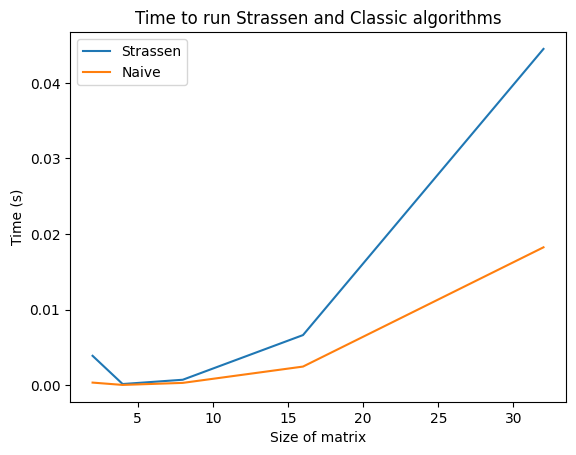
\includegraphics[width=0.6\textwidth, height=7.8cm]{figs/time_2.png}
    \caption{Time Complexity of Strassen's Algorithm and Classical Method}
\end{figure}

\begin{figure}[htbp]
    \centering
    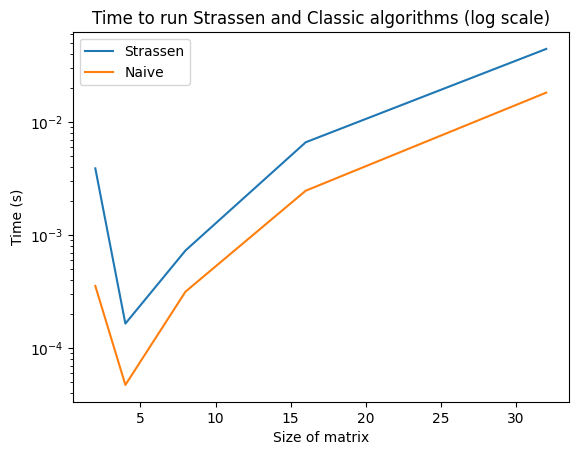
\includegraphics[width=0.6\textwidth, height=7.8cm]{figs/log_time_2.png}
    \caption{Time Complexity of Strassen's Algorithm and Classical Method(log scale)}
\end{figure}
In order to compare the performance of Strassen's algorithm and the classical method, we implement both of them in Python and compare the time they cost to do the matrix multiplication.
We test the running time of both Strassen's algorithm and the classical method for matrix with size of exponetial of $2$ from $2^1$ to $2^{5}$. From the figures shown above, we can see that the classical method
has a generally good performance than Strassen's algorithm when the size of the matrix is relative small. However, when the size of the matrix is large enough, Strassen's algorithm has a better performance than the classical method.

\begin{figure}[h!]
    \centering
    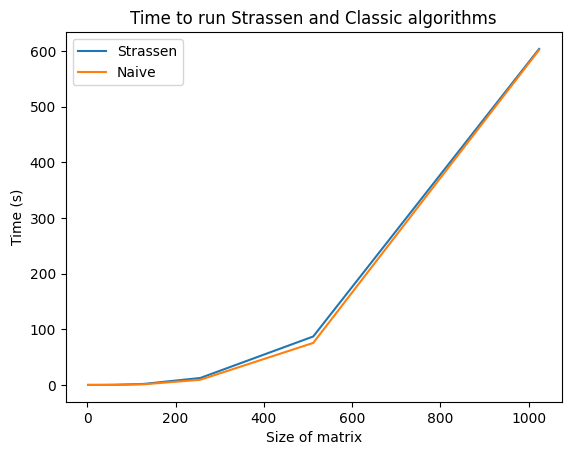
\includegraphics[width=0.6\textwidth, height=7.8cm]{figs/time.png}
    \caption{Time Complexity of Strassen's Algorithm and Classical Method with Larger Size of Matrix}
\end{figure}
\begin{figure}[h!]
    \centering
    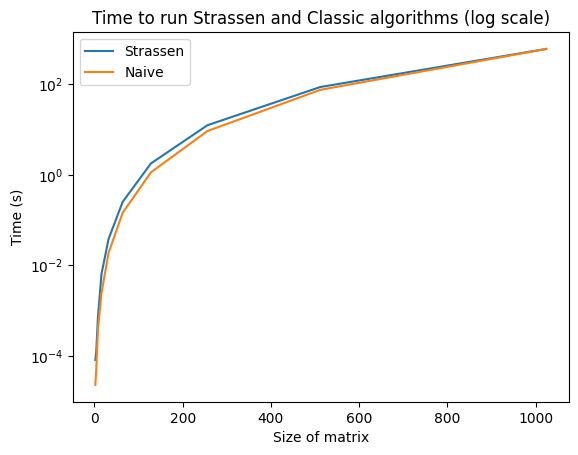
\includegraphics[width=0.6\textwidth, height=7.8cm]{figs/log_time.png}
    \caption{Time Complexity of Strassen's Algorithm and Classical Method with Larger Size of Matrix(log scale)}
\end{figure}

Then we do the experiment for the size of the matrix from $2^1$ to $2^{10}$. From the figures 3 and 4, we can see the time used by Strassen's algorithm becomes closer to the time used by the classical method. 
And when the size of the matrix is large enough, Strassen's algorithm has a better performance than the classical method. From figure 5, we can observe that as the matrix's size n become over 2000, the time used
by classical method become much more than the time used by Strassen's algorithm.\\

\begin{figure}[h!]
    \centering
    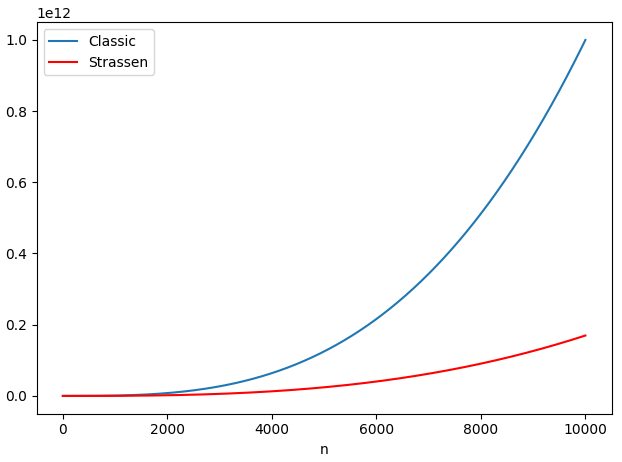
\includegraphics[width=0.6\textwidth, height=7.8cm]{figs/time_3.png}
    \caption{Time Complexity of Strassen's Algorithm and Classical Method}
\end{figure}

\begin{figure}[h!]
    \centering
    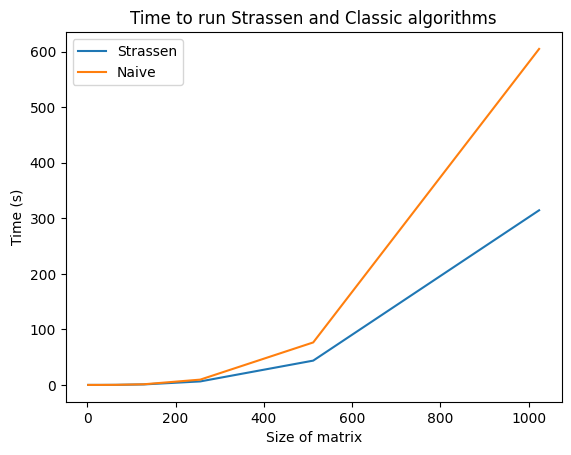
\includegraphics[width=0.6\textwidth, height=7.8cm]{figs/time_4.png}
    \caption{Time Complexity of Strassen's Algorithm with Threshold and Classical Method}
\end{figure}

Thus the choice becomes very important. Intuitively, we can try to understand the concept in this way. If we have a matrix with size 10000 by 10000, then it's 
useful to divide it into small matrices and do few additions and subtractions. However, if we have a matrix with size 10 by 10, it's not necessary to divide it into small matrices.\\
\begin{figure}[h!]
    \centering
    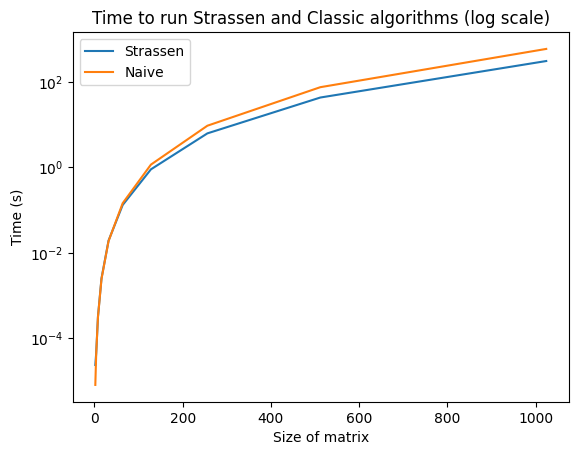
\includegraphics[width=0.6\textwidth, height=7.8cm]{figs/log_time_4.png}
    \caption{Time Complexity of Strassen's Algorithm with Threshold and Classical Method(log scale)}
\end{figure}

The basic takeaway from this experiment
is that we can add a threshold to decide whether we should use Strassen's algorithm or the classical method which means when we do Strassen's algorithm recursively as the matrices are split into a sufficiently small size we 
should directly use classical methed to calculate instead of waiting it split the matrix into size of 1.\\

In figure 6 and 7, they plot the comparison of the time used by Strassen's algorithm with threshold and the classical method. The threshold used is 32 which means for the matrix with size less than 32 by 32, we will use 
classical method instead of Strassen's algorithm. Still for the matrices with size from $2^1$ to $2^{10}$, now the time used by Strassen's algorithm with threshold is much less than the time used by the classical method.\\

In conclusion, although asymptotically Strassen's algorithm is faster than the classical method, it doesn't mean Strassen's algorithm is faster, the constant factors involved in Strassen's algorithm are larger than those 
in the classical method. So in practice, when implementing Strassen's algorithm, we should be careful about the size of the matrix we are dealing with, and it's always a good idea to add a threshold to decide whether we 
should use Strassen's algorithm or the classical method which can save a lot of time when dealing with small matrices.

\section{Limitation of Strassen Algorithm in Stability}
\hspace{5.5mm}Strassen's algorithm is not quite as numerically stable as the classical method. Strassen's algorithm only concerns dense matrices and that the matrices need to be fairly large for it to be worthwhile. As what introduced in the
previous section, the computers use floating point arithmetic to do the calculation which means the result of the calculation is not as accurate as what we compute by hand. And the error will be accumulated as the calculation 
goes on, especially for the Strassen's algorithm we recursively do the calculation. So the result of the Strassen's algorithm is not as accurate as we expect it to be.\\

\section{Conclusion and Discussion}
\end{document}